\documentclass{beamer} % papier A4
\usepackage[utf8]{inputenc}      % accents dans le source
\usepackage[T1]{fontenc}         % accents dans le pdf
\usepackage{textcomp}            % symboles complémentaires (euro)
\usepackage[frenchb]{babel}      % titres en français
\usepackage{amsmath}
\usepackage{amsthm}
\usepackage{amssymb}
\usepackage{algorithm}
\usepackage{algorithmic}
\usepackage{pgf}
\usepackage{tikz}
\usepackage{tikz-cd}
\usepackage{rotating}
\usepackage{framed}
\usepackage{xcolor}
\usepackage{color}
\usetikzlibrary{matrix,arrows,decorations.pathmorphing}
\usepackage{array}
\usepackage{caption}
\usepackage{graphicx, wrapfig}
\numberwithin{equation}{section}
\usepackage{multicol}
\setbeamertemplate{theorems}[numbered]
% Maccros pour les commandes de math
\newcommand\nroot[1]{\textit{#1}-ième}
\newcommand\zmodn[1]{\mathbb{Z}/#1\mathbb{Z}}
\newcommand\zmodninv[1]{(\mathbb{Z}/#1\mathbb{Z})^{\times}}
\newcommand\GF[1]{\mathbb{F}_{#1}}
\newcommand\Irr[2]{\textup{Irr}_{#1}(#2)}
\newcommand\Tr[1]{\textup{Tr}\left(#1\right)}
\newcommand\QQ{\mathbb{Q}}
\newcommand\ZZ{\mathbb{Z}}
\newcommand\NN{\mathbb{N}}
\newcommand\CC{\mathbb{C}}
\newcommand\RR{\mathbb{R}}
\newcommand\EO{\mathcal{O}}
\newcommand\PP[1]{\mathbb{P}^{#1}}
\newcommand\etmath{\textup{\quad et \quad}}
\newcommand\M[1]{\textup{M}(#1)}
\newcommand\E[1]{\textup{E}(#1)}
\newcommand\I[1]{\textup{I}(#1)}
\newcommand\tO[1]{\widetilde{O}(#1)}
\newcommand\groupgen[1]{\langle{#1}\rangle}
% Algorithmic en français
\floatname{algorithm}{Algorithme}
\renewcommand{\algorithmicrequire}{\textbf{Entrée :}}
\renewcommand{\algorithmicensure}{\textbf{Sortie :}}
\renewcommand{\algorithmiccomment}[1]{\{#1\}}
\renewcommand{\algorithmicend}{\textbf{fin}}
\renewcommand{\algorithmicif}{\textbf{si}}
\renewcommand{\algorithmicthen}{\textbf{alors}}
\renewcommand{\algorithmicelse}{\textbf{sinon}}
\renewcommand{\algorithmicelsif}{\algorithmicelse\ \algorithmicif}
\renewcommand{\algorithmicendif}{\algorithmicend\ \algorithmicif}
\renewcommand{\algorithmicfor}{\textbf{pour}}
\renewcommand{\algorithmicforall}{\textbf{pour tout}}
\renewcommand{\algorithmicdo}{\textbf{faire}}
\renewcommand{\algorithmicendfor}{\algorithmicend\ \algorithmicfor}
\renewcommand{\algorithmicwhile}{\textbf{tant que}}
\renewcommand{\algorithmicrepeat}{\textbf{répéter}}
\renewcommand{\algorithmicuntil}{\textbf{jusqu'à}}
\renewcommand{\algorithmicreturn}{\textbf{renvoyer}}
\renewcommand{\algorithmicto}{\textbf{à}}
\newcommand\ord[2]{\textup{ord}_{#1}(#2)}
\setbeamerfont{page number in head/foot}{size=\large}
\setbeamertemplate{footline}[frame number]
\definecolor{elliptique}{HTML}{B22222}
\definecolor{o1}{HTML}{32CD32}
\definecolor{o2}{HTML}{1E90FF}
\definecolor{o3}{HTML}{9932CC}
\definecolor{o4}{HTML}{00FFFF}
\definecolor{o6}{HTML}{D2691E}
\begin{document}
\title{Calcul d'isomorphismes de corps finis}
\author{Ludovic Brieulle}
\newtheorem*{thm}{Thèorème}
\newtheorem{lem}{Lemme}
\newtheorem{cor}{Corollaire}
\newtheorem{prop}{Proposition}
\theoremstyle{definition}
\newtheorem{defn}{Définition}
\newtheorem*{ex}{Exemple}
\theoremstyle{remark}
\newtheorem*{rem}{Remarque}
\newtheorem*{conj}{Conjecture}
\tikzstyle{every picture}+=[remember picture]
\everymath{\displaystyle}





\begin{frame}
\begin{titlepage}
\emph{Encadré par :}
Luca \bsc{De Feo} (PRiSM, UVSQ), % Supervisor's Name
Jean-Pierre \bsc{Flori} (ANSSI), % Supervisor's Name
Jérôme \bsc{Plût} (ANSSI)% Supervisor's Name
\begin{center}

\includegraphics[scale=0.3]{Anssi}
\hspace{3cm}

\includegraphics[scale=0.2]{UVSQ}
\end{center}
\end{titlepage}
\end{frame}
\section{Introduction}
\begin{frame}
\frametitle{Introduction}
\textbf{Objectif du stage :}\\
Étudier et implanter sur \bsc{SAGE} une variante d'un algorithme jamais
implantée avant et la comparer à des algorithmes déjà existant pour 
calculer un isomorphisme de corps finis.
\begin{table}
\centering
\begin{tabular}{|l|c|}
	\hline
	Méthode & Complexité\\
	\hline\hline
	Cyclotomique et elliptique (Pinch, 1991) & $-$\\
	\hline
	Cyclotomique (Rains, 1996) & $\tO{n^2}$\\
	\hline
	Algébre linéaire (Allombert, 2002) & $\tO{n^2}$\\
	\hline
	Elliptique (variante de Rains) & $\tO{n^2}$\\
	\hline
\end{tabular}
\end{table}
		

\end{frame}
%1
\begin{frame}
\frametitle{Introduction}
\framesubtitle{Énoncé}
Soit $p$ premier, soit $q =p^r$ et $n$ un entier.\\
$\GF{q^n}$ \og{le}\fg{} corps à $q^n$ éléments, unique à \emph{isomorphisme
près}.\\
\textbf{Données :}
\begin{itemize}
\item $f,g\in\GF{q}[X]$ irréductibles de degré $n$,
\item $k_1 := \GF{q}[X]/(f)\etmath k_2 := \GF{q}[Y]/(g)$.
\end{itemize}
\textbf{Problème :}\\
Construire un isomorphisme
\[\theta : k_1 \buildrel\sim\over\longrightarrow k_2.\]
c'est-à-dire, déterminer l'image du générateur $x$ de $k_1$.

\end{frame}
%2
\begin{frame}
\frametitle{Introduction}
\framesubtitle{Solution naïve}
\textbf{Solution naïve :}
Trouver une racine de $f$ dans $k_2$.\\
Complexité : $\tO{n^2}$ (factoriser un polynôme dans $\GF{q}$)\\
\emph{Problème :} lent en pratique.\\
\vspace{0.3cm}
\textbf{Autre solution :}
Trouver deux éléments définissant un isomorphisme et en déduire l'image de
$x$.\\
C'est-à-dire, trouver deux éléments $\alpha$ et $\beta$ ayant le même polynôme 
minimal : 
\[\textup{min}_{\GF{q}}(\alpha) = \textup{min}_{\GF{q}}(\beta)\]
\end{frame}
\section{Pinch}
%3
\begin{frame}
\frametitle{Méthode de Pinch cyclotomique (1991)}
\tikzstyle{na} = [baseline=-.5ex]
Soit $\mu_m$ le groupe des racines $m$-ièmes de l'unité.\\
Soit $\Phi_m$ le polynôme minimal des générateurs $\zeta_m$ de $\mu_m$, les 
racines \emph{primitives} $m$-ièmes de l'unité.\\
\vspace{0.3cm}
\textbf{Données :}
\begin{itemize}
	\item $\GF{q^n}^{\times}$ le groupe multiplicatif de $\GF{q^n}$,
	\item $m$ un entier tel que les $\zeta_m$ engendrent $\GF{q^n}$.
\end{itemize}
\vspace{0.3cm}
\textbf{Objectif :}\\
Exprimer $\zeta_m$ dans $k_1$ et $k_2$ pour déduire des deux expresisons l'image
de $x$ en fonction de $y$.
\end{frame}
\begin{frame}
\frametitle{Méthode de Pinch cyclotomique (1991)}
\textbf{Procédure :}
\begin{itemize}
	\item Calculer $\zeta_m\in k_1$ et $\zeta'_m\in k_2$,
\item \textbf{Si} $\Phi_m$ est irréductible sur $\GF{q}$ :
\begin{itemize}
	\item Inverser la matrice de passage de la base $(\zeta_m^i)$ à la base
$((\zeta_m^{\prime})^i)$ et en déduire l'image de $x$.
\end{itemize}
\vspace{0.3cm}
\item \textbf{Sinon :}\\
\begin{equation*}
\Phi_m(X) = \tikz[baseline]{\node[anchor=base] (t1) {$P_1(X)$};} \dots 
\tikz[baseline]{\node[anchor=base] (t2) {$P_i(X)$};}  
\tikz[baseline]{\node[] (t3) {$\dots$};} P_e(X)
\end{equation*}
\hspace{3.5cm}
$\tikz\node [] (n1) {$\zeta'_m$};$
\hspace{0.8cm}
$\tikz\node [] (n2) {$\zeta_m$};$
\hspace{0.3cm}
$\tikz\node [] (n3) {$(\zeta'_m)^{s}$};$
\begin{tikzpicture}[overlay]
        \path[->,>=angle 90] (n1) edge [] (t1);
        \path[->,>=angle 90] (n2) edge [] (t2);
        \path[->,>=angle 90] (n3) edge [] (t3);
\end{tikzpicture}
	\begin{itemize}
	\item Trouver $0 < s < \varphi(m)$ tel que $\zeta_m$ et $(\zeta'_m)^s$ aient
le même polynôme minimal.
	\item Inverser la matrice de passage de la base $(\zeta_m^i)$ à la base
$((\zeta_m^{\prime})^{si})$ et en déduire l'image de $x$.
	\end{itemize}
\end{itemize}


\end{frame}
\begin{frame}
\frametitle{Méthode de Pinch}
\textbf{Problèmes :}
\begin{itemize}
	\item Taille de $m$, au pire la complexité peut être exponentielle en $n$
(p. ex. si $l = q^n - 1$)
	\item $\Phi_m$ réductible sur la plupart des corps finis, tester plusieurs
$s$ avant de tomber sur un isomorphisme.
\end{itemize}
\textbf{Solutions :}
\begin{itemize}
	\item Utiliser des extensions pour diminuer la taille de $m$.
	\item Générer des éléments ayant le même polynôme minimal.
\end{itemize}
\end{frame}
\section{Méthode de Rains cyclotomique}
%5
\begin{frame}
\frametitle{Méthode de Rains cyclotomique (1996)}
\tikzstyle{na} = [baseline=-.5ex]
\textbf{Données :}
\begin{itemize}
	\item $\GF{q^n}^{\times}$ le groupe multiplicatif de $\GF{q^n}$
	\item $m$ un entier tel que $\groupgen{q}$ soit l'unique sous-groupe d'ordre
$n$ dans $\zmodninv{m}$.
\end{itemize}
\vspace{0.3cm}
\textbf{Objectif :}
Générer deux éléments ayant le même polynôme minimal, ces éléments s'appellent
\emph{périodes de Gauss}.
\end{frame}
\begin{frame}
\frametitle{Méthode de Rains cyclotomique (1996)}
\tikzstyle{na} = [baseline=-.5ex]
\begin{framed}
\begin{thm}
Soient $\eta_1$ et $\eta_2$ définis comme ci-dessous, alors ils engendrent
$\GF{q^n}$ et 
\[\textup{min}_{\GF{q}}(\eta_1) = \textup{min}_{\GF{q}}(\eta_2)\]
\end{thm}
\end{framed}
Soient $\zeta_m\in k_1$ et $\zeta'_m\in k_2$ :
\begin{equation*}
\Phi_m(X) = \tikz[baseline]{\node[anchor=base] (t1) {$P_1(X)$};} \dots 
\tikz[baseline]{\node[anchor=base] (t2) {$P_i(X)$};}
\dots P_e(X)
\end{equation*}
\hspace{4cm}
$\tikz\node [] (n1) {$\zeta'_m$};$
\hspace{0.8cm}
$\tikz\node [] (n2) {$\zeta_m$};$

\begin{tikzpicture}[overlay]
        \path[->,>=angle 90] (n1) edge [] (t1);
        \path[->,>=angle 90] (n2) edge [] (t2);
\end{tikzpicture}
Soit $S$ le sous-groupe de $\zmodninv{m}$ tel que $\zmodninv{m} = 
\groupgen{q}\times S$. Les périodes de Gauss de $\zeta_m$ et $\zeta'_m$ sont :
\[
\eta_1 = \sum_{\sigma\in S}{\zeta_m^{\sigma}}\etmath
\eta_2 = \sum_{\sigma\in S}{(\zeta'_m)^{\sigma}}
\]
\end{frame}
%6
\begin{frame}
\frametitle{Méthode de Rains cyclotomique (1996)}
\textbf{Algorithme :}\\
Entrée :
\begin{itemize}
	\item $k_1$, $k_2$, extensions de degré $n$ de $\GF{q}$,
	\item $m$ un entier tel que $\groupgen{q}$ soit l'unique sous-groupe 
		d'ordre $n$ de $\zmodninv{m}$.
\end{itemize}
Sortie :\\
\begin{itemize}
\item $\eta_1$ et $\eta_2$ tels que $\textup{min}_{\GF{q}}(\eta_1) =
\textup{min}_{\GF{q}}(\eta_2)$.
\end{itemize}
\begin{enumerate}
	\item Calculer $\zeta_m\in k_1$ et $\zeta'_m\in k_2$
	\item Calculer $\eta_1$ et $\eta_2$.
\end{enumerate}
\vspace{0.5cm}
\emph{Complexité} : $\tO{n^2}$\\
\end{frame}
\begin{frame}[fragile]
\frametitle{Méthode de Rains cyclotomique (1996)}
\textbf{Extension :}\\
Si $m$ est trop grand, on utilise une extension de degré $o$.
\begin{center}
\begin{tikzpicture}
\matrix(m)[matrix of math nodes,
row sep=3em, column sep=3em,
text height=1.5ex, text depth=0.25ex]
{\GF{q}[\eta(\zeta_m)] & \GF{q}[\eta(\zeta'_m)]\\
\GF{q}[\Tr{\eta(\zeta_m)}] & \GF{q}[\Tr{\eta(\zeta'_m)}]\\};
\path[->,font=\scriptsize,>=angle 90]
(m-1-1) edge node[auto] {} (m-1-2)
(m-2-1) edge node[auto] {$\theta$} (m-2-2);
\path[-,font=\scriptsize,>=angle 90]
(m-1-1) edge node[left] {$o$} (m-2-1)
(m-1-2) edge node[right] {$o$} (m-2-2);
\end{tikzpicture}
\end{center}
\vspace{0.3cm}
\emph{Complexité :} $\tO{(no)^2}$\\
\textbf{Problème :} Construire une extension coûte très cher.
\end{frame}
%7
\section{Méthode elliptique de Rains}
\begin{frame}
\frametitle{Variante elliptique de Rains}
\textbf{Données :}
\begin{itemize}
	\item $E/\GF{q}$ une courbe elliptique,
	\item $m$ un entier tel que l'abscisse des points de $m$-torsion de $E$
engendrent $\GF{q^n}$.
\end{itemize}
\vspace{0.3cm}
\textbf{Périodes elliptiques: }\\
\[\eta_{\alpha}(P)=\sum_{\sigma\in S}{([\sigma]P)_X}\]
où $P_X$ est l'abscisse d'un poit $P$, $\alpha$ valeur propre du Frobenius de
$E/\GF{q}$ d'ordre $n$ modulo $m$ et $S$ sous-groupe de $\zmodninv{m}$ tel que :
\[\zmodninv{m} = \groupgen{\alpha}\times S\]
\end{frame}
\begin{frame}
\frametitle{Variante elliptique de Rains}
\begin{framed}
\begin{conj}
Pour tout $P$ d'ordre exactement $m$, les $\eta_{\alpha}(P)$ engendrent 
$\GF{q^n}$ et ont tous le même polynôme minimal.
\end{conj}
\end{framed}
\begin{table}
\begin{tabular}{|c|c|}
\hline
Méthode cyclotomique & $\,$$\,$Méthode elliptique$\,$$\,$\\
\hline
\hline
$\GF{q^n}^{\times}$ & $E/\GF{q^n}$\\
\hline
$\mu_m$ & $E[m]$\\
\hline
$\eta(\zeta_m)$ & $\eta_{\alpha}(P)$\\
\hline
$\tO{n^2}$ & $\tO{n^2}$\\
\hline
\end{tabular}
\end{table}
\end{frame}
\section{Implantation}
\begin{frame}
\frametitle{Implantation}
\textbf{Détails de l'implantation :}\\
\begin{itemize}
\item Langage : SAGE (python)
\item Paramètres : $q = p$, $n$ premier, $m$ premier
\end{itemize}

\end{frame}
\begin{frame}
\frametitle{Comparaison}
\begin{figure}
\begin{center}
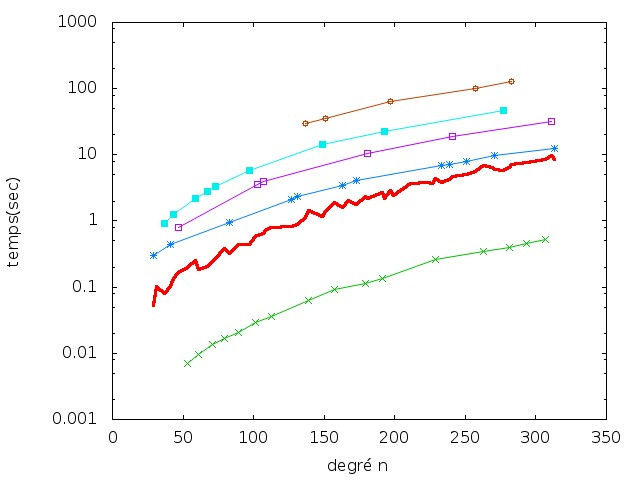
\includegraphics[scale=0.5]{testrc3}
\caption*{\scriptsize Comparaison de la méthode elliptique
(\textcolor{elliptique}{$+$}) avec la méthode cyclotomique $o = 1$
 (\textcolor{o1}{$\times$}), $o = 2$ (\textcolor{o2}{$*$}), $o = 3$ 
(\textcolor{o3}{$\Box$}), $o = 4$ (\textcolor{o4}{$\blacksquare$}), $o = 6$ 
(\textcolor{o6}{$\diamond$}) en fonction du degré $n$, pour $p = 101$}
\end{center}
\end{figure}

\end{frame}
\section{Conclusion}
\begin{frame}
\frametitle{Conclusion}
\textbf{Résultats :}
\begin{itemize}
	\item Nouvelle algorithme,
	\item Résultats compétitifs,
	\item Possible intégration dans \bsc{SAGE}.
\end{itemize}
\vspace{0.3cm}
\textbf{Futurs objectifs :}
\begin{itemize}
	\item Cas général ($q$ puissance d'un nombre premier, $n$ et $m$ composés),
	\item Deuxième partie du problème.
\end{itemize}
\end{frame}
\end{document}
